\documentclass[border=4pt]{standalone}
% Shared by the independently buildable vector figures.
\usepackage[T1]{fontenc}
\usepackage{amsmath,amssymb,newpxtext,newpxmath}
\usepackage[semibold]{sourcesans}
\usepackage{pgfplots}
\pgfplotsset{compat=1.18}
\usetikzlibrary{arrows.meta,calc,positioning}
\usepgfplotslibrary{groupplots}
\definecolor{ink}{HTML}{19303A}
\definecolor{sea}{HTML}{00675E}
\definecolor{clay}{HTML}{A24725}
\definecolor{muted}{HTML}{4C636C}
\definecolor{rulegray}{HTML}{CAD4D4}
\definecolor{wash}{HTML}{EAF4F0}
\definecolor{warm}{HTML}{F7EEE5}
\color{ink}
\tikzset{every picture/.style={font=\sffamily\small},
  arrow/.style={-{Stealth[length=2mm]},line width=.8pt,draw=muted}}
\pgfplotsset{companion/.style={axis lines=left,axis line style={draw=muted},
  tick style={draw=muted},ticklabel style={font=\sffamily\footnotesize,text=muted},
  label style={font=\sffamily\small},grid=major,grid style={draw=rulegray!64,line width=.25pt},
  tick align=outside,enlarge x limits=false,scaled ticks=false,
  every axis plot/.append style={line join=round},
  legend style={draw=none,fill=none,font=\sffamily\footnotesize},
  title style={font=\sffamily\bfseries\small,anchor=south west,at={(0,1.03)}}}}

\begin{document}
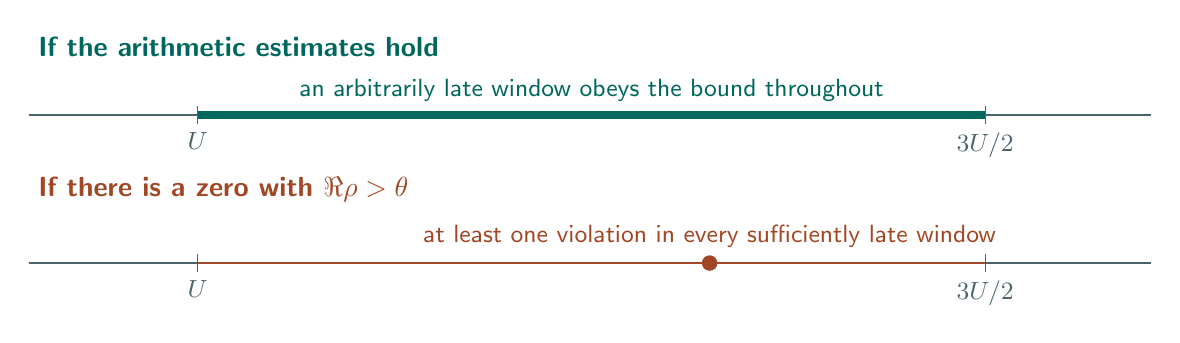
\begin{tikzpicture}[x=1cm,y=1cm]
\node[anchor=west,font=\sffamily\bfseries,text=sea] at (0,2.9){If the arithmetic estimates hold};
\node[anchor=west,font=\sffamily\bfseries,text=clay] at (0,1.08){If there is a zero with $\Re\rho>\theta$};
\foreach \y in {2.03,.15}{
  \draw[muted,line width=.6pt] (0,\y) -- (14.25,\y);
  \draw[muted] (2.15,\y-.12) -- (2.15,\y+.12);
  \draw[muted] (12.15,\y-.12) -- (12.15,\y+.12);
  \node[below,text=muted] at (2.15,\y-.1) {$U$};
  \node[below,text=muted] at (12.15,\y-.1) {$3U/2$};
}
\draw[sea,line width=3pt] (2.15,2.03)--(12.15,2.03);
\node[above,text=sea] at (7.15,2.08){an arbitrarily late window obeys the bound throughout};
\draw[clay,line width=.9pt] (2.15,.15)--(12.15,.15);
\fill[clay] (8.65,.15) circle (2.8pt);
\node[above,text=clay] at (8.65,.23){at least one violation in every sufficiently late window};
\end{tikzpicture}
\end{document}
